%%%%%%%%%%%%%%%%%%%%%%%%%%%%%%%%%%%%%%%%%%%%%%%%%%%%%%%%%%%%%%%%%%%%%%%%%%%%%%%
% Autor: 
	% Christian Hinrichs, 2013--2015; 
	% Arash Shahbakhsh, 2018, Anpassung LUH-EI; 
	% Paul Hendrik Tiemann, 2018; 
	% Stephan Ferenz 2019-2020
	% Arash Shahbakhsh, Herbst 2020, Anpassung uol-des  
%%%%%%%%%%%%%%%%%%%%%%%%%%%%%%%%%%%%%%%%%%%%%%%%%%%%%%%%%%%%%%%%%%%%%%%%%%%%%%%
\documentclass[
11pt,                                                  % Schriftgroesse fuer Abschlussarbeiten: 11 pt (Vorgabe))
BCOR=10mm,                                              % ca. 280 Seiten = 140 Blätter * 0.14 mm / 2 = Bindekorrektur 10 mm > will correct page margins!
DIV=12,                                                % Textspiegel: Zwölferteilung (siehe Beschreibung KOMA-Script)
twoside=true,                                          % Dokument zweiseitig setzen?
headinclude=true,                                      % Kopfzeile zum Textkörper zählen?
footinclude=false,                                     % Fußzeile zum Textkörper zählen?
a4paper,                                               % Papierformat zur Berechnung des Satzspiegels
pagesize=auto,                                         % Papierformat des Kompilates gemäß 'paper' setzen
parskip=false,                                         % Absatzauszeichnung: 1 em Einzug, kein Abstand
numbers=noenddot,                                      % Gliederungsnummern mit Punkt? (auto = Duden-Vorschrift)
%Mapping=tex-text        
cleardoublepage=empty,                                 % Vakatseiten komplett leer
open=right,                                            % Kapitel immer auf rechter Doppelseite beginnen
chapterprefix=false,                                   % Präfix "Kapitel 1" vor Kapitelüberschrift?
appendixprefix=false,                                  % Präfix "Anhang A" vor Anhangüberschrift?
numbers=noenddot,                                      % Gliederungsnummern mit Punkt? (auto = Duden-Vorschrift)
% leqno,                                               % Gleichungen links statt rechts nummerieren
fleqn,                                                 % Gleichungen linksbündig statt zentriert ausgeben
toc=bib,                                               % Literaturverzeichnis im Inhaltsverzeichnis
toc=listof,                                            % Abbildungs- und Tabellenverzeichnis (so vorhanden) im Inhaltsverzeichnis 
]{scrreprt}                                            % scrreprt, da scrbook keine abstract-Umgebung hat

% ----------------------------- Import settings -------------------------------

%Pakete für Seitenformat
\usepackage[automark]{scrlayer-scrpage}
%\usepackage{scrlayer-scrpage}

% For colors
\usepackage[dvipsnames]{xcolor}

% Paket zum Platzieren von Hintergrundgrafiken (fuer Uni-Logo auf Deckblat verwendet)
\usepackage{eso-pic}
\newcommand\AtPageUpperRight[1]{\AtPageUpperLeft{\makebox[\paperwidth][r]{#1}}}

%Pakete für Schriften
\usepackage[utf8]{inputenc}
\usepackage[T1]{fontenc}

%Paket für das Euro-Zeichen
\usepackage{eurosym}

%Pakete für Sprache
\usepackage[english,ngerman]{babel} %Using main= does not work with hyperref (autoref). Please set the main language by writing it last in [].

%Pakete für Listings
\usepackage{listings}
\usepackage{scrhack}		% to remove warning from srcreprt

%Pakete für Grafiken
\usepackage[pdftex]{graphicx}
\usepackage{pdflscape} % pdf-Grafiken quer auf eine Seite
\usepackage{caption}
%\usepackage{subcaption}
\usepackage{subfig} % Grafiken mit mehreren Abbildungen

%Pakete fuer Tabellen
\usepackage{tabularx}

%Mathematik-Pakete
\usepackage{amssymb}
\usepackage{amsmath}
\usepackage{amsthm}
\usepackage{cancel}

%Anklickbares Verzeichnis für PDF
\usepackage{hyperref}

%Akronyme
\usepackage{acronym}

%Pakete für die Bibliographie
\usepackage{bibgerm}
\usepackage{url}
\usepackage{float}
\usepackage{floatflt}
\usepackage{array}
\usepackage{fancybox}
\usepackage{framed}
\usepackage{wasysym}
\usepackage{pifont}
\def\UrlBreaks{\do\/\do-}

%Pakete zum Auskommentieren
\usepackage{afterpage}

% Paket fuer Ueberschriften in Tabellen
\usepackage{makecell}
\renewcommand\theadalign{cc} % t,c,b and l,c,r for top, center, bottom and left, center and right
\renewcommand\theadfont{\bfseries}
\renewcommand\theadgape{\Gape[4pt]}
\renewcommand\cellgape{\Gape[4pt]}

% Paket für Todo's
\usepackage[colorinlistoftodos]{todonotes} 
%\usepackage[colorinlistoftodos, disable]{todonotes}% ich glaube ausschalten mit: disable

% For lists
\usepackage{enumitem} %% To change the position of items

% For headings etc:
% classicthesis & arsclassica
\usepackage{scrtime}
\usepackage{textcase}

% For nomenclature
\usepackage[intoc, german, noprefix]{nomencl}

% For import of pdf_tex
\usepackage{import}

% For long tables on multiple pages:
\usepackage{longtable}

% Tabelle centering
\usepackage{tabulary}

% Package to better adjust page margins
\usepackage{geometry}

% Package necessary for Cref definition
\usepackage[nameinlink]{cleveref}

% for vanishing the error of scalable font
\usepackage[T1]{fontenc}
\usepackage{lmodern}

\newcommand{\documentauthor}{Name hier einfügen (variables.tex)}     % Hier Namen eintragen
\newcommand{\documentauthorbirthday}{01.01.1990}
\newcommand{\documentauthorbirthplace}{Oldenburg}

\newcommand{\documenttitle}{
	Titel der Arbeit (variables.tex)
}
\newcommand{\documentgrade}{Master of Science}
%\newcommand{\documentcourse}{Elektro- und Informationstechnik}
\newcommand{\documentcourse}{Wirtschaftsingenieur}

\newcommand{\documentfaculties}{
	Fakultät II - Department für Informatik}
%\newcommand{\documentfaculties}{
%Fakultät für Elektrotechnik und Informatik, Fakultät für Maschinenbau und
%der Wirtschaftswissenschaftlichen Fakultät \\ der Leibniz Universität Hannover}
\newcommand{\documentinstitute}{
\iflanguage{ngerman}
	{Abteilung für Digitalisierte Energiesysteme}
	{Faculty II - Department of Informatics\\ Digitalisierte Energiesysteme}
}
\newcommand{\documentuniversity}{
%	Gottfried Wilhelm Leibniz Universität Hannover, Deutschland\\
	Carl von Ossietzky Universität Oldenburg
}

\newcommand{\documenttutori}{%
	Prof. Dr.-Ing. Astrid Nieße
}
\newcommand{\documenttutorii}{%
	Prof. Dr.-Ing. \#2 (variables.tex) 
}
\newcommand{\documentsupervisor}{
	M.Sc. (Dr.-Ing.) \#3
}

\newcommand{\documenttutor}{%
	Erstprüferin: \documenttutori \\
	Zweitprüfer: \documenttutorii \\
	Betreuerin: \documentsupervisor \\
}

%fuer Deckblatt und Erklaerung am Ende auf Deutsch
\newcommand{\documentdate}{\today}
\newcommand{\documenttype}{Masterarbeit}
\newcommand{\documentlocation}{Oldenburg}

%fuer hypersetup - Metainfos und Verlinkung innerhalb des Dokuments
\newcommand{\documentsubject}{Energietechnik, Energiespeicher, Leibniz Universität Hannover,
	Masterarbeit, Lastmanagement, Spitzenlastkappung, Atypik}
\newcommand{\documentkeywords}{Energiespeicher, Lastspitzen, Netzentgelt}


%% Packages
\usepackage{a4wide}
\usepackage{ifthen}
%
\usepackage[ngerman,english]{babel} %Using main= does not work with hyperref (autoref). Therefore, the main language the later one and main is not used!
\usepackage[utf8]{inputenc}
\usepackage[T1]{fontenc}
\usepackage{ae,aecompl}
\usepackage{graphicx}
\usepackage{tabularx}
\usepackage{pgfgantt}	% used for the timetable
\usepackage{hyperref}	% for \url and other refs

\usepackage[nameinlink]{cleveref} % Package necessary for Cref definition

\usepackage{cleveref} % for improved footnotes with reuseable lables
\crefformat{footnote}{#2\footnotemark[#1]#3}

\usepackage[hyphenbreaks]{breakurl}	% Break urls

%% Setup
\hypersetup{colorlinks=true,
	linkcolor=cyan,
	citecolor=cyan,
	urlcolor=cyan} % No color frame but color links instead

%% Commands
% Funktion to get doi as link when using bmc-mathphys.bst
\newcommand*{\doiurl}[1]{\href{http://doi.org/#1}{#1}}

% Set Margins
\topmargin 0cm \textheight 23cm \parindent0cm

% Renew enumeration
\renewcommand{\labelenumii}{\theenumii} % Strcture mit 1. 2. statt a) b)
\renewcommand{\theenumii}{\theenumi.\arabic{enumii}.}
\renewcommand{\labelenumiii}{\theenumiii} % dritte Ebene
\renewcommand{\theenumiii}{\theenumi.\arabic{enumii}.\arabic{enumiii}.}


% deactivate citep
%\newcommand{\citep}[1]{\cite{#1}}
% Text rot/gruen faerben
\newcommand{\red}[1]{\textcolor{red}{\textbf{#1}}}
\newcommand{\recheck}[1]{ \colorbox{green}{\textbf{#1}} }
% Verkürzen des Kommandos für tiefgestellten Text
\newcommand{\tsub}[1]{\textsubscript{#1}}
% Anführungszeichen oben und unten
\newcommand{\gqq}[1]{\glqq #1\grqq}
% Exponentialfunktion mit e
\newcommand{\ex}{{\textrm e}} 

% Definition TODOs:
\newcommand{\todoAsk}[2][]{\todo[color=yellow!50,#1]{\textcolor{red}{Ask for:} #2}}
\newcommand{\todoFormulate}[2][]{\todo[color=lightgray,#1]{\textcolor{red}{Formulate:} #2}}

% missing [...]
\newcommand{\missing}{ \colorbox{red}{\textbf{...}} }


\newcommand{\items}[1]{
	~\vspace{0.2cm}\\
	\framebox[\textwidth]{
		\begin{tabular}{m{1.2cm}m{14cm}}
			\includegraphics[height=1cm]{Pics/gp.jpg} &
			\begin{itemize}#1\end{itemize}
		\end{tabular}
	}
	~\vspace{0.2cm}\\
}

% Abbildungen
%\newcommand{\image}[2]{
%	\begin{figure}[h]
%		\begin{center}
%			\includegraphics{Pics/#1}
%			\caption{#2}
%		\end{center}
%	\end{figure}
%}

\newcommand{\image}[2]{
	\begin{figure}[h]
		\begin{center}
			\includegraphics{Pics/#1}
			\vspace{-0.2cm}
			\caption{#2}
		\end{center}
	\end{figure}
}

\newcommand{\imagewithtext}[3]{
	\begin{figure}[h]
		\begin{center}
			\includegraphics{Pics/#1}
			\caption{#2}
			~\\
			#3
		\end{center}
	\end{figure}
}

\newcommand{\fullsizeimage}[2]{
	\begin{figure}[h]
		\begin{center}
			\includegraphics[width=\textwidth]{Pics/#1}
			\caption{#2}
		\end{center}
	\end{figure}
}



%Workaround für \lstlistoflistings
\makeatletter
\@ifundefined{float@listhead}{}{%
    \renewcommand*{\lstlistoflistings}{%
        \begingroup
    	    \if@twocolumn
                \@restonecoltrue\onecolumn
            \else
                \@restonecolfalse
            \fi
            \float@listhead{\lstlistlistingname}%
            \setlength{\parskip}{\z@}%
            \setlength{\parindent}{\z@}%
            \setlength{\parfillskip}{\z@ \@plus 1fil}%
            \@starttoc{lol}%
            \if@restonecol\twocolumn\fi
        \endgroup
    }%
}
\makeatother

%\let\oldlstlisting=\lstlisting
%\def\lstlisting{\vspace{-0.5cm}\oldlstlisting}

% Funktion to get doi as link when using bmc-mathphys.bst
\newcommand*{\doiurl}[1]{\href{http://doi.org/#1}{\detokenize{#1}}}

%Redefine some autorefs:
\addto\extrasenglish{
	\renewcommand{\subsectionautorefname}{section}
}

%Set figure to be lower case for autoref
\addto\extrasenglish{%
	\renewcommand{\figureautorefname}{figure}%
}
\addto\extrasenglish{%
	\renewcommand{\tableautorefname}{table}%
}


%For fancy nomenclature
\makenomenclature
% Mehrere nomencl-Abschnitte:
% http://www.mrunix.de/forums/showpost.php?p=210422&postcount=29
\renewcommand{\nomname}{Abbreviations}
\renewcommand{\nompreamble}{\markboth{\nomname}{\nomname}}
\renewcommand{\nomlabelwidth}{2.5cm}
\newcommand{\nomaltname}{Nomenclature}
\newcommand{\nomaltpreamble}{\markboth{\nomaltname}{\nomaltname}}
\newcommand{\nomaltpostamble}{}
\newcommand{\switchnomitem}{S}
\renewcommand{\nomgroup}[1]{%
	\ifthenelse{\equal{#1}{\switchnomitem}}{\switchnomalt}{}}
\newcommand{\switchnomalt}{%
\end{thenomenclature}
\renewcommand{\nomname}{\nomaltname}
\renewcommand{\nompreamble}{\nomaltpreamble}
\renewcommand{\nompostamble}{\nomaltpostamble}
\begin{thenomenclature}
}

\recalctypearea % Satzspiegel neu berechnen (damit Seitenraender eingestellt werden)

% -- eigene Variablen, z.B. fuer Gleichungen

% Laenge des Hochlastzeitfensters
\newcommand{\THLZ}{T^{\textrm{HLZ}}}
% Vorladezeit
\newcommand{\Tvorl}{T^{\textrm{vorl}}}



% richtige Silbentrennung erzwingen, nur falls notwendig
\hyphenation{Selbst-ent-ladung Un-ter-neh-mens-pro-zesse}
\hyphenation{kur-zen Netz-ebe-ne Abs-zisse Un-ste-tig-keits-stel-le}
\hyphenation{Ins-ti-tut In-te-res-se da-raus}

%% For version 2 of Acronyms
%%%%%%%%%%%%%%%%%%%%%%%%%%%%%%%%%%%%%%%%%%%%%%%%%%%%%%%%%%%%%%%%%%%%%%%%%%%%%%%%
% Autor: Christian Hinrichs, 2013--2015, Stephan Ferenz 2019
%%%%%%%%%%%%%%%%%%%%%%%%%%%%%%%%%%%%%%%%%%%%%%%%%%%%%%%%%%%%%%%%%%%%%%%%%%%%%%%
% Abbreviations and general terms
%
\newcommand{\bspw}{bspw.}
\newcommand{\Bspw}{Bspw.}

%
%%%%%%%%%%%%%%%%%%%%%%%%%%%%%%%%%%%%%%%%%%%%%%%%%%%%%%%%%%%%%%%%%%%%%%%%%%%%%%%
% Acronyms
%
\makeatletter
\newcommand{\mkacr}[2]{%
  % #1 = the acronym
  % #2 = definition of the acronym
  %
  % Example:
  % \mkacr{KWK}{Kraft-Wärme-Kopplung}
  % This will do the following:
  % - Create a command "\KWK" that expands to "\textsf{KWK}"
  % - Create a tooltip over the expanded text,
  %   containing "Definition: Kraft-Wärme-Kopplung"
  % - Create command \xKWK just like above, but without tooltip
  % - Create an entry in the nomenclature (list of acronyms, nomencl package
  %   required) using the string "Kraft-Wärme-Kopplung" from argument #2
  %		> You need to generate the right nls file by running "\makeindex mainThesis.nlo -s nomencl.ist -o mainThesis.nls" in terminal
  %
  % Define the actual command
  \global\expandafter\DeclareRobustCommand\csname #1\endcsname{%
    \href{Definition: #2}{%
    	\textcolor{black}{\textsf{#1}}%
    }%
  }%
  % The same for the "\x..." variant without tooltip
  \global\expandafter\DeclareRobustCommand\csname x#1\endcsname{%
    \textsf{#1}
  }%
  %
  % Finally, create the nomenclature entry (nomencl package required)
  \nomenclature[A#1]{\textsf{#1}}{#2}
}
\makeatother
%
% -----------------------------------------------------------------------------
% Es folgen einige Beispielakronyme zur Veranschaulichung:
%
% Standard Acronyms:
%% FunktionenEnergieversorgung
\mkacr{DER}{Distributed Energy Resources}
\mkacr{RQ}{Research Question}


%
% Sepcials (which require either a special command name, or a special tooltip):
% \newcommand{\PtoP}{%
%   \href{Definition: Peer-to-Peer Netz}{%
%     \textcolor{black}{\textsf{P2P}}%
%   }%
% }
% \nomenclature[AP2P]{\textsf{P2P}}{Peer-to-Peer Netz}
%
%
%
%%%%%%%%%%%%%%%%%%%%%%%%%%%%%%%%%%%%%%%%%%%%%%%%%%%%%%%%%%%%%%%%%%%%%%%%%%%%%%%
% Symbols
%
% For symbols, we usually cannot use the symbol itself as command name, so that
% must be customizable. Also, we want to be able to assign an index to the
% symbols. Thus the command definition below is a lot more difficult.
%
\makeatletter
\newcommand{\mksym}[4]{%
  % #1 = command name for the symbol
  % #2 = the symbol itself
  % #3 = definition of the symbol
  % #4 = definition of the prefix, for nomenclature sorting. May be left empty.
  %
  % Example:
  % \mksym{sfit}{v}{Güte}{11g}
  % This will do the following:
  % - Create a command "\sfit" that expands to "v" in math mode,
  %   or to "$v$" in text mode
  % - Create a command "\sfit[i]" that expands to "v_{i}" or "$v_{i}$",
  %   where "i" is an arbitrary argument
  % - Create a tooltip over the expanded symbol, containing "Definition: Güte"
  % - Create commands \xsfit and \xsfit[i] just like above, but without tooltip
  % - Create an entry in the nomenclature (list of symbols, nomencl package
  %   required) using the string "Güte" from argument #3 and the sorting prefix
  %   from argument #4
  %
  % First, define delegates for optional argument handling
  \global\expandafter\DeclareRobustCommand\csname #1\endcsname{%
    \@ifnextchar[%
      {\csname @@#1\endcsname}% with some argument [foo]
      {\csname @#1\endcsname}% without argument
  }%
  % The same for the "\x..." variant without tooltip
  \global\expandafter\DeclareRobustCommand\csname x#1\endcsname{%
    \@ifnextchar[%
      {\csname @@x#1\endcsname}% with some argument [foo]
      {\csname @x#1\endcsname}% without argument
  }%
  %
  % Second, build the actual delegate targets (hyperref package required)
  \global\expandafter\def\csname @@#1\endcsname[##1]{%
    \ensuremath{%
      \textrm{%
        \href{Definition: #3}{%
          \textcolor{black}{\ensuremath{#2}}%
        }%
      }%
      _{##1}%
    }%
  }%
  \global\expandafter\def\csname @#1\endcsname{%
    \textrm{%
      \href{Definition: #3}{%
        \textcolor{black}{\ensuremath{#2}}%
      }%
    }%
  }%
  \global\expandafter\def\csname @@x#1\endcsname[##1]{%
    \ensuremath{#2_{##1}}%
  }%
  \global\expandafter\def\csname @x#1\endcsname{%
    \ensuremath{#2}%
  }%
  %
  % Finally, create the nomenclature entry (nomencl package required)
  \nomenclature[S#4]{\ensuremath{#2}}{#3}%\hspace*{-1.5cm}#3}
}
\newcommand{\mksymNom}[4]{%
	% Finally, create the nomenclature entry (nomencl package required)
	\nomenclature[S#4]{\ensuremath{#2}}{#3}%\hspace*{-1.5cm}#3}
}
\newcommand{\mksymhref}[4]{%
	% #1 = command name for the symbol
	% #2 = the symbol itself
	% #3 = definition of the symbol
	% #4 = definition of the prefix, for nomenclature sorting. May be left empty.
	%
	% Example:
	% \mksym{sfit}{v}{Güte}{11g}
	% This will do the following:
	% - Create a command "\sfit" that expands to "v" in math mode,
	%   or to "$v$" in text mode
	% - Create a command "\sfit[i]" that expands to "v_{i}" or "$v_{i}$",
	%   where "i" is an arbitrary argument
	% - Create a tooltip over the expanded symbol, containing "Definition: Güte"
	% - Create commands \xsfit and \xsfit[i] just like above, but without tooltip
	% - Create an entry in the nomenclature (list of symbols, nomencl package
	%   required) using the string "Güte" from argument #3 and the sorting prefix
	%   from argument #4
	%
	% First, define delegates for optional argument handling
	\global\expandafter\DeclareRobustCommand\csname #1\endcsname{%
		\@ifnextchar[%
		{\csname @@#1\endcsname}% with some argument [foo]
		{\csname @#1\endcsname}% without argument
	}%
	% The same for the "\x..." variant without tooltip
	\global\expandafter\DeclareRobustCommand\csname x#1\endcsname{%
		\@ifnextchar[%
		{\csname @@x#1\endcsname}% with some argument [foo]
		{\csname @x#1\endcsname}% without argument
	}%
	%
	% Second, build the actual delegate targets (hyperref package required)
	\global\expandafter\def\csname @@#1\endcsname[##1]{%
		\ensuremath{%
			\textrm{%
				\href{Definition: #3}{%
					\textcolor{black}{\ensuremath{#2}}%
				}%
			}%
			_{##1}%
		}%
	}%
	\global\expandafter\def\csname @#1\endcsname{%
		\textrm{%
			\href{Definition: #3}{%
				\textcolor{black}{\ensuremath{#2}}%
			}%
		}%
	}%
	\global\expandafter\def\csname @@x#1\endcsname[##1]{%
		\ensuremath{#2_{##1}}%
	}%
	\global\expandafter\def\csname @x#1\endcsname{%
		\ensuremath{#2}%
	}%
	%
	% Without nom entry
}
\makeatother
%
% Declare \mathsfit as sans-serif + non-bold + italic in math mode,
% using the Kp font
\DeclareMathAlphabet{\mathsfit}{\encodingdefault}{jkpss}{m}{it}
%
% -----------------------------------------------------------------------------
% Es folgen einige Beispielsymbole zur Veranschaulichung:
%
% Symbols: Allgemein
\nomenclature[S00]{\textbf{\textsf{Latin Symbols}}}{}
\mksym{P}{P}{Active power}{0}
\mksym{Q}{Q}{Reactive power}{0}


\nomenclature[S20]{\textbf{\textsf{Indices}}}{}
\mksym{ind}{ind}{Inductive}{2}
\mksym{capi}{cap}{Capacitive}{2}

%
\nomenclature[S30]{\textbf{\textsf{Agreements}}}{}
\mksym{PFcos}{\cos(\varphi)}{Power factor}{3}

\begin{document}
\pagestyle{empty}
\pagenumbering{roman}
%----------------------------- TITLE PAGE -------------------------------------
% Grundsaetzlich bitte Vorgaben der jeweiligen Pruefungsordnungen beachten
\begin{titlepage}
\newgeometry{left=3cm,right=3cm}

%%%%%%%%%%%%%%%%%%%%%%%%%%%%%%%%%%%%%%%%%%%% UOL-Logo
 \AddToShipoutPictureBG*{\AtPageUpperRight{\raisebox{-3.6cm}{
\includegraphics[width=167px]{images/des_logo}\hspace{2cm}}}}

%%%%%%%%%%%%%%%%%%%%%%%%%%%%%%%%%%%%%%%%%%%% DES-Logo
\AddToShipoutPictureBG*{\AtPageUpperLeft{\raisebox{-3.6cm}{\hspace{2cm}
\includegraphics[width=110px,clip]{images/uol_logo}}}}


\begin{center}
\vspace*{4cm}

   %\begin{figure}[h]
   %		\centering
   %		\includegraphics[height=4cm]{images/welfenschloss_vektor}
   %\end{figure}

    {\large \textsc{\documentuniversity}}\\
    {\large \textsc{\documentinstitute}} \\[1.2cm]
	
    {\LARGE{\textbf{\documenttitle}}} \\[1.2cm]
    {\Large{\textbf{\documenttype}}} \\[0.4cm]
    %\textnormal{\iflanguage{ngerman}{zur Erlangung des akademischen Grades "`\documentgrade"' im Studiengang \documentcourse ~der \documentfaculties}{to reach the academic degree "\documentgrade" in major \documentcourse ~ at the\documentfaculties}} \\ [0.4cm]

	\iflanguage{ngerman}{vorgelegt von}{submitted by} \\ [0.4cm]
    {\Large \textbf{\documentauthor}} \\ [0.4cm]
    \iflanguage{ngerman}{Geboren am {\documentauthorbirthday} in {\documentauthorbirthplace} }{born on {\documentauthorbirthday} in {\documentauthorbirthplace} } \\ [2cm]

    \begin{tabular}{ll}%rl
      \iflanguage{ngerman}{Erstprüferin:}{First Examiner:}  		& \documenttutori \\
      \iflanguage{ngerman}{Zweitprüfer:}{Second Examiner:}  		& \documenttutorii \\
      \iflanguage{ngerman}{Betreuer:}{Supervisor:}    		& \documentsupervisor \\
    \end{tabular} \\ [1.2cm]

    \large{\textnormal{\documentlocation, \iflanguage{ngerman}{den \documentdate}{\documentdate}}}
\end{center}

\restoregeometry
\end{titlepage} % detailliertes Deckblatt

%-------------------------- END OF TITLE PAGE ---------------------------------
\microtypesetup{protrusion=false}
\pagestyle{plain} 
%\thispagestyle{empty}

\begin{abstract} % unterdrueckt u.a. Kopf- und Fusszeile
\begin{center}
 % empty line
\begin{minipage}{12cm}
\iflanguage{ngerman}{\textit{Kurzzusammenfassung}}{\textit{Abstract}}\\
Hier ist Platz für die Kurzzusammenfassung (Abstract) der Arbeit. Die Kurzzusammenfassung sollte maximal eine Seite lang sein und in der Regel in der selben Sprache verfasst sein wie die Arbeit. 
Sofern die Arbeit nicht in Englisch geschrieben wurde, ist es natürlich möglich auch noch zusätzlich eine Englische Zusammenfassung zu erstellen.

\end{minipage}
\end{center}
\end{abstract}
 

% optional: ACKNOWLEDGEMENT
%\input{content/acknowledgement.tex}

% -------------------------- TABLE OF CONTENTS --------------------------------
\cleardoublepage
\pdfbookmark{\contentsname}{toc} % Adds content to the internal content list of the pdf
\tableofcontents

% -------------------------- ACRONYMS & NOMENCLATURE --------------------------
% Two versions for acronyms are provided:
% Version 1: A simple one using Acronyms.tex and Nomenclature.tex
% Version 2: A more complicated one with better support for more hyperlinks using acronymsV2.tex

% Version 1
\newcommand{\acrTitle}{\iflanguage{ngerman}{Abkürzungen}{Abbreviations}}

\chapter*{\acrTitle}
\addcontentsline{toc}{chapter}{\acrTitle}

\begin{acronym}[SpeicherSpikaAtypik]
	% sorting in alphabetical order manually!!!
	
	%	\acro{acronym}{full name}
	%	\acroplural{acronym}[short plural name]{full plural name}
	
	\acro{DES}{Abteilung für Digitalisierte Energiesysteme}
	\acro{IfES}{Institut für Elektrische Energiesysteme}
	\acro{NB}{Netzbetreiber}
	\acro{NNE}{Netznutzungsentgelt}
	\acroplural{NNE}[NNE]{Netzentgelte}
	\acro{StromNEV}{Stromnetzentgeltverordnung}
	\acro{StromNZV}{Stromnetzzugangsverordnung}
	\acro{VEA}{VEA Bundesverband der Energieabnehmer e.V.}
	
\end{acronym}

\newpage

\newcommand{\nomTitle}{\iflanguage{ngerman}{Formelzeichen}{Nomenclature}} % is used as title of the chapter and for the table of contents

\chapter*{\nomTitle}
\addcontentsline{toc}{chapter}{\nomTitle}
%
In der Arbeit verwendete Formelzeichen, Symbole und Indizes sind tabellarisch aufzulisten. Die Reihenfolge ist alphabetisch, getrennt nach lateinischen und griechischen Buchstaben. Je nach Art der Arbeit, ist ggf. auch eine weitere Trennung nach hochgestellten/tiefgestellten Indizes, skalaren/vektoriellen Größen usw. sinnvoll. Weiterhin kann es sinnvoll sein spezielle packages für die Erstellung des Formelzeichenverzeichnisses zu verwenden, ähnlich wie für Abkürzungen.

\begin{acronym}[Formelzeichen]
	% sorting in alphabetical order manually!!!
	
	\acro{pi}[\ensuremath{\pi}]{Die Zahl Pi}
	\acro{alpha}[\ensuremath{\alpha}]{Das Symbol alpha}

	
\end{acronym}


\newpage

%% Version 2
%\printnomenclature  

% ----------------------------- Prepare for Content  --------------------------
\microtypesetup{protrusion=true}
\cleardoublepage
\pagenumbering{arabic}
\pagestyle{scrheadings} 
% ---------------------------- CONTENT ----------------------------------------
\chapter{Template für Abschlussarbeiten}
\label{chap:template}

This template is intended for all theses written in the Digitized Energy Systems Group. The most important instructions for the use of this template are given within this text.

To this end, \autoref{chap:changes} first describes various parameters, some of which you need to change or some of which you may change.

Then, \autoref{chap:recommendations} presents some recommendations for a good thesis.

In the last chapter, \autoref{chap:examples} presents various functionalities of Latex as examples.

If questions arise about the use of this template that cannot be solved with Google, feel free to contact your supervisor.
\chapter{changes to be made}
\label{chap:changes}

This chapter introduces variables you should change to use this template.
For this purpose, \autoref{sec:necessary_changes} first describes the mandatory parameters.  After that, \autoref{sec:optional_changes} deals with some settings that you may changes to according to your own preference.

\section{Mandatory Parameters}
\label{sec:necessary_changes}

This section contains the aspects which you definitely need change, please read it thoroughly.

\subsection{variables.tex}
In \textit{config/variables.tex} many important parameters can be adjusted for your work, including:
\begin{itemize}
	\item title
	\item author (including birthplace and birthday)
	\item second examiner
	\item type of thesis
	\item keywords of the thesis
\end{itemize}
It makes sense to adjust everything accordingly.

\subsection{language}
If your thesis is not written in German, it is worth changing the language. This can be done in \textit{config/packages.tex}. There the main language should be passed as the last argument for the package \textit{Babel}.
The titles of the sections (incl. table of contents, table of figures etc.), graphics and tables as well as the title page and the explanation at the end will change the language. (At least for German and English this should work).


\section{Optional Changes}
\label{sec:optional_changes}
This section introduces more advanced settings that you can change if needed.

\subsection{Customize the color of the links}
The color of the links can be changed in the \textit{config/config.tex} file. Here \textit{linkcolor} is defined as the color of all links in the PDF.
For printing this can be changed to the color 'black'.

\subsection{Changing the bibliography}
You can change the style of the bibliography. For this you can change the \textit{bibliographystyle} in \textit{main.tex}. A few suggestions are already stored there.

\subsection{Change to single page printing}
In the \textit{main.tex} at the beginning you can change \textit{twoside} to \textit{false} to create a one-sided output.
\chapter{recommendations}
\label{chap:recommendations}

We generally have the following recommendations for theses:

\section{General}
\begin{itemize}
	\item All tables and figures included in the thesis should be referenced in the text. Tables and figures should generally be inserted in the text approximately where they are referenced. For technical referencing in the PDF file, see \autoref{sec:ref}.
	\item For figures either high-resolution images or vector graphics (e.g. PDFs, SVGs) should be used.
	\item There should be no line break between number and unit. A protected space can be used here, which can be inserted in Latex via the tilde~\textasciitilde~. The same applies to references of any form (figure~x, table~y, etc.).
\end{itemize}

\section{Mathematical symbols}
Formula characters should be formatted as follows:
\begin{itemize}
	\item variables: italic
	\item constants: steep (\textit{textrm} command in math environment).
	\item count indices: italic
	\item Indices: steep
	\item Complex numbers: underlined
\end{itemize}
Mathematical operators should also be steeply formatted.
\chapter{examples}
\label{chap:examples}

This chapter presents examples for some functionalities of Latex.
Of course, there is no claim to completeness, since Latex offers many different possibilities to perform additional formatting and to include other files.

First, \autoref{sec:tables_imgs} introduces ways to insert tables and images. Afterwards \autoref{sec:code} presents how to best include source code in your work.
After that, \autoref{sec:ref} is about referencing things. After that \autoref{sec:lit} briefly shows how to cite sources correctly with Latex. Other small features are introduced in \autoref{sec:other}.

The chapter concludes with an example introduction in \autoref{sec:example_intro}.

\section{images and tables}
\label{sec:tables_imgs}
\begin{figure}
	\centering
	\subfloat[Centralized control]{
		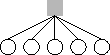
\includegraphics[width=\textwidth*2/5]{img_examples/Control_centralized.pdf}
	}
	\subfloat[Proper hierarchical control]{
		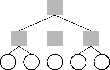
\includegraphics[width=\textwidth*2/5]{img_examples/Control_hierarchical.pdf}
	}\\
	\subfloat[Modified hierarchical control]{
		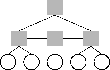
\includegraphics[width=\textwidth*2/5]{img_examples/Control_hierarchical_modified.pdf}
	}
	\subfloat[Heterarchical (distributed) control]{
		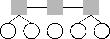
\includegraphics[width=\textwidth*2/5]{img_examples/Control_heterarchical.pdf}
	}
	\caption{Different forms of control architecture, where the control components are represented by boxes and the circles serve as controllable units, based on \cite{dilts_evolution_1991}}
	\label{Fig:ControlArch}
\end{figure}

In \autoref{Fig:ControlArch} you will see an illustration with several sub-illustrations, each of which will be included as \textit{pdf}. \textit{png} files as well as other image files can be included in the same way.

\begin{figure}
	\centering
	\def\svgwidth{\textwidth*5/11}
	\import{img_examples/}{MV.pdf_tex}
	\caption[Mandatory operating area in the MV grid, based on \cite{vde_vde-ar-n_2018-1}]{Mandatory operating area in the MV grid, based on \cite{vde_vde-ar-n_2018-1}}
	\label{Fig:MVOperating}
\end{figure}

In \autoref{Fig:MVOperating} is an example for including \textit{pdf\_tex} files, where tex-text can also be stored. Various other software, e.g., Inkscape can create such files.

\begin{table}
	\centering
	\begin{tabular}{m {3cm} | *{4}{c|} m{2.5cm}}
		Devices & \multicolumn{2}{c|}{Active power demand} & \multicolumn{2}{c|}{Reactive power demand} & Others \\
		& Increase & Decrease & Increase & Decrease & \\
		\hline
		\hline
		Inverter-based generators & + & & + & + & \\hline
		Conventional power plants & + & & + & + & Regulation of voltage level \\\hline
		Static reacitve compensating devices & & & + & + & \\\hline
		Under-load tap-changing transformers & & & & & Change of voltage level at one side \\\hline
		Energy storage systems & & + & + & + & \\hline
		Loads & & + &&&
	\end{tabular}
	\caption{Overview of devices which can support voltage regulation and their capability to increase or decrease their active or reactive power demand or to help voltage regulation in another way}
	\label{Tab:DevVolReg}
\end{table}

In \autoref{Tab:DevVolReg} you can see an example table with table caption.

\section{Source Code}
\label{sec:code}

Source code can be displayed using the \href{https://www.ctan.org/pkg/listings}{listings} package.

\begin{lstlisting}[caption=examplecode,language=python]
	def factorial(n):
	"""Program to calculate the factorial of a positive integer"""
	if n < 0:
	raise ValueError("You must enter a positive number")
	
	fact = 1
	i = 2
	while i <= n:
	fact = fact * i
	i += 1
	
	print(fact)
\end{lstlisting}

In addition to directly including the source code, a file can also be read in:
\begin{lstlisting}{name}
	\lstinputlisting[frame=single,label=examplecode,caption=anexample]{example.py}
\end{lstlisting}

\section{References}
\label{sec:ref}

There are several ways to create references.

\subsection{References to other text sections, images or tables}
First, a \textit{label} must be created to be referenced.
With \textit{ref} you can create a reference to a label with only a number, e.g. see \ref{sec:ref}. With \textit{autoref} the type label is added, e.g. see \autoref{sec:ref}. For English it is useful to use the command \textit{Cref} at the beginning of the sentence to enable proper capitalization, e.g. see \Cref{sec:ref}.

\subsection{References to the internet}
Two commands can be used to link to the Internet. With \textit{url} the URL is also displayed as text, e.g. \url{www.uol.de/des}.
With \textit{href} any text can be chosen, e.g. \href{www.uol.de/des}{Digitized energy systems}.

\section{Acronyms}
\label{sec:abbrev}
The package \textit{acronym} is used for acronyms.
The acronyms should be introduced in \textit{content/Acronyms.tex}. There are a few examples in that file. These can be included in the following way:
\begin{itemize}
	\item \textit{ac}: First mention with definition, after that only short vresion
	\item \textit{acp}: Similar to \textit{ac} but with plural
	\item \textit{acs}: Only gives the short form
\end{itemize}

The package can also be used for a list of symbols (see \textit{content/Nomenclature.tex} as example).

There is a second variant to define acronyms in \textit{content/acronymsV2.tex} which is more advanced and not compatible with overleaf. Therefore, we recommend the use of this variant only for advanced LaTeX users.

If you want to use the second option the following changes are necessary for this:
\begin{enumerate}
	\item The first option for acronyms in the \textit{main.tex} need to be commented and the second version need to be included.
	\item Instead of \textit{content/Acronyms.tex} and \textit{content/Nomenclature.tex} the other nomenclature from \textit{content/acronymsV2.tex} is now used.
	\item When compiling the PDF, \textit{\textbackslash makeindex mainThesis.nlo -s nomencl.ist -o mainThesis.nls} should be run in the terminal.
\end{enumerate}

\section{Literature}
\label{sec:lit}

In a scientific paper, assumptions must be proved. In addition, an examination of the current state of scientific research is relevant. For this purpose, appropriate sources should be cited.

For referencing sources, there is \href{https://de.wikipedia.org/wiki/BibTeX}{bibtex} in latex.
The relevant information about publications (author, title, year, etc.) is collected in the file \textit{bib/Literature.bib}. Literature management software, such as \href{https://www.citavi.com/de}{citavi} and \href{https://www.zotero.org/}{zotero}, offer an export to the format directly and also on literature websites a corresponding export of the relevant metadata is usually possible.

If you want to cite a source, it is sufficient to use the \textit{cite} command and put the identifier of the source (which can be found in the literature file at the beginning of each source) in the curly brackets.
The source will be automatically added to the bibliography.



For programming, which is often part of a thesis, mostly already existing software tools are used. If there are scientific publications about them, they should be included in the bibliography. References to the web pages of the software tools belong (including the version number and the date of retrieval) in a footnote\footnote{example: \url{https://mosaik.offis.de/}, Mosaic version: 2.5.1, accessed 2019-07-12}.

\section{sec:other}
\label{sec:other}

This section is about various small packages that may be useful.
\subsection{ToDo-Notes}
ToDo-Notes can be used to create small to-dos. The general documentation can be found at \url{https://www.ctan.org/pkg/todonotes}.
\todo[inline]{ToDos can be created \textit{inline} by specifying the additional option \textit{inline}}
\todoAsk{Normally, however, the ToDos are in the margin}
At the end of the PDF, a list of all ToDos is created.
The package is included in \textit{config/packages.tex} and all ToDos can be disabled with the \textit{disable} option.
Additional ToDo types can be created in \textit{config/commands.tex} where you can find an example.


\section{Beispieleinleitung}
\label{sec:example_intro}
Die Wettbewerbsfähigkeit energieintensiver Industrien beruht wesentlich auf einem erfolgreichen Kostenmanagement.
Die Energieausgaben bei der Herstellung sowie beim Umschlag und Transport von Gütern belasten deren Budget.
Laut Strompreisanalyse des Bundesverbandes der Energie- und Wasserwirtschaft~e.V. (2017) ist der Industriestrompreis seit dem Jahr~2000 von 6,05~ct/kWh auf 17,12~ct/kWh angestiegen (siehe Abbildung~\ref{fig:Strompr}).
Daher suchen insbesondere industrielle Betriebe sowie andere energieintensive Einrichtungen wie etwa Krankenhäuser nach Wegen, um diese Aufwendungen zu verringern.
\begin{figure}[b!]
	\centering
		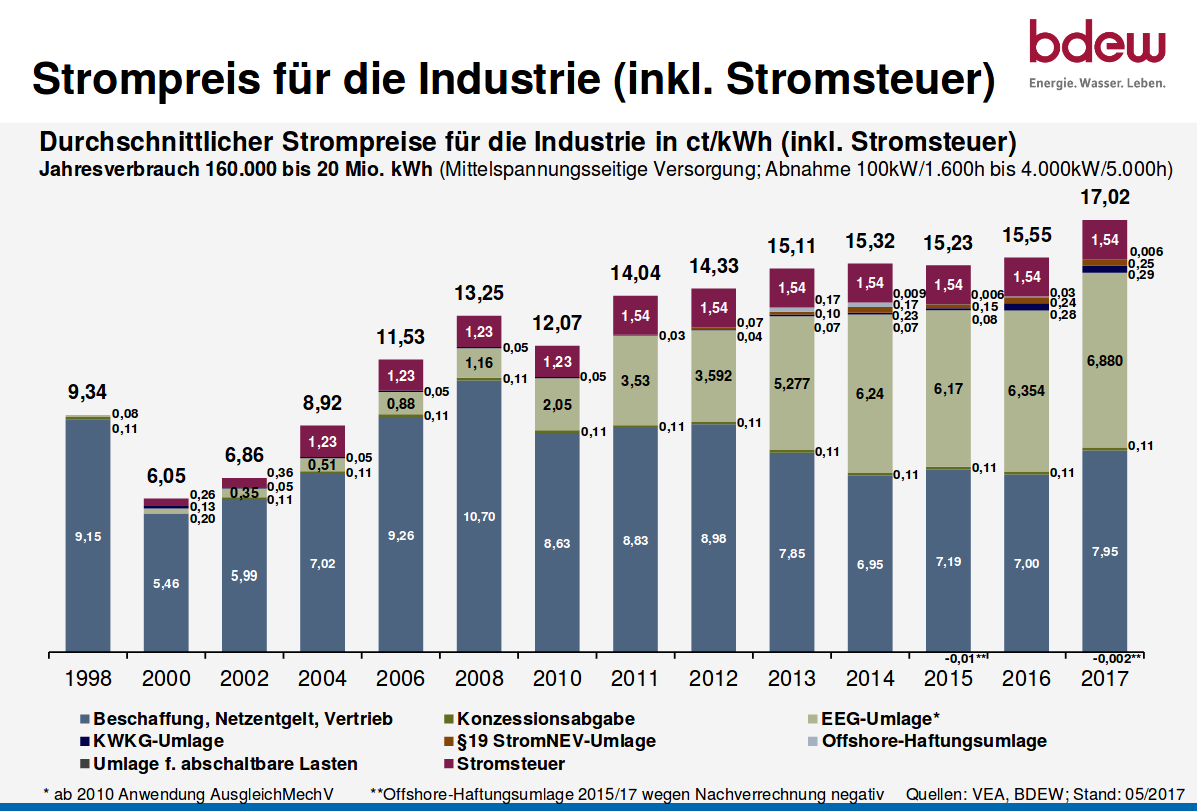
\includegraphics[width=\textwidth]{img_examples/BDEWStrompreis.png}
		\caption[Strompreisentwicklung BDEW]{Entwicklung des Strompreises für die Industrie in Deutschland von 1998 bis 2017 \cite{BDEWMai17}.		}
		\label{fig:Strompr}
\end{figure}
Beispielsweise wurden Möglichkeiten gefunden, durch eine optimierte Energiebeschaffung, durch Anwendung der \gqq{besonderen Ausgleichsregelung} \footnote{Durch die besondere Ausgleichsregelung können sich Unternehmen aus stromkosten- und handelsintensiv eingestuften Branchen von der Zahlung eines Teils der EEG-Umlage befreien lassen.}, durch Steuerbefreiung sowie durch Eigenstromerzeugung Kosten zu senken.
Verursacht durch den Netzausbau zur Aufnahme alternativer Energien steigen die Netznutzungsentgelte (NNE) seit 2011 erheblich.
\begin{figure}[tb!]
	\centering
		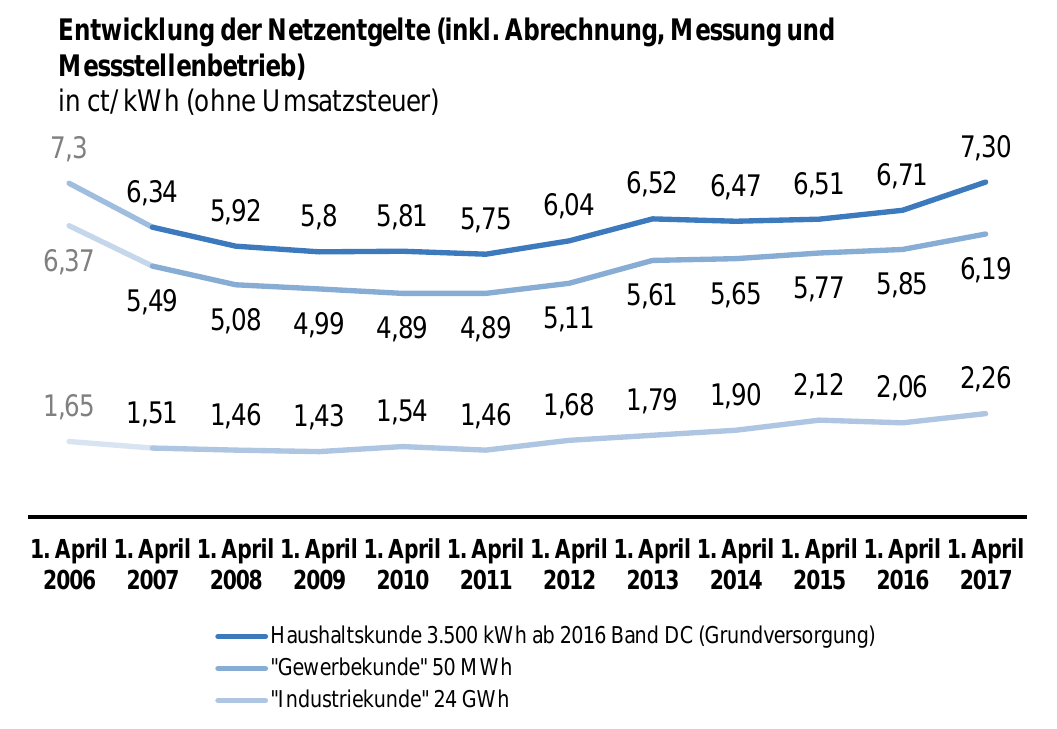
\includegraphics[width=12cm]{img_examples/BNetzANNE17.png}
		\caption[Netzentgeltentwicklung BNetzA]{Entwicklung der \aclp{NNE} in Deutschland von 2006 bis 2017 \cite{Monitor17}.
		}
		\label{fig:NNEEnt}
\end{figure}
Zwischenzeitlich waren diese seit der Einführung der Anreizregulierung im Jahr 2006 gefallen (siehe Abbildung~\ref{fig:NNEEnt}).
Daher ist es für die Industrie existenziell wichtig, Wege zur \ac{NNE}-Reduktion zu analysieren oder wenigstens ihr Potenzial für Entlastungen abzuschätzen.
Die Systematik zur Berechnung von Netzentgelten bietet für Unternehmen mit leistungsgemessen Abnahmestellen Möglichkeiten, ihre Kosten zu reduzieren.
Danach ist ein leistungsabhängiger Anteil zu entrichten, der vom maximalen Netzbezug im Abrechnungszeitraum abhängt.
Dieser wirkt sich stark auf die zu entrichtenden Beträge aus.
Aufgrund dieser Berechnungsweise des Netzentgeltes ist es wichtig, zu bestimmten Zeiten die dem Netz gegenüber an einem Anschlusspunkt auftretende Last zu reduzieren.
Anzustreben ist entweder ein verringertes allgemeines Netzentgelt oder ein niedriges individuelles Netzentgelt nach §~19~\ac{StromNEV}.
Diese unterscheiden sich dadurch, zu welchen Zeiten und in welchem Umfang Leistungsspitzen reduziert werden sollen.
%
%
\subsection{Anlass und Arbeitshypothesen der Untersuchung}
\label{Ansatz}
Durch eine Kooperation des \ac{VEA} mit dem \ac{IfES} der Leibniz Universität Hannover entstand ein Interesse, das Potenzial eines Speichereinsatzes für die deutsche Industrie genauer zu untersuchen.
Der \ac{VEA} hat dafür einen Zugriff auf sein EDV-System mit Unternehmensdatensätzen und Lastprofilen gewährt.
Im Verband sind viele energieintensive Firmen des deutschen Mittelstandes vertreten.
So kann davon ausgegangen werden, dass Ergebnisse einer solchen Untersuchung auf der Basis verfügbarer Daten repräsentativ sind für die deutsche Industrie.
Gleichzeitig steht ein vom \ac{IfES} entwickeltes Simulationsprogramm zur Verfügung, in dem Energiespeicher verschiedener Technologien einheitlich beschrieben sind.
Mithilfe der Lastgangdaten kann deren Kapazität dimensioniert und die Wirtschaftlichkeit untersucht werden.
Insgesamt waren zum Bearbeitungszeitpunkt der vorliegenden Studie vollständige Datensätze von 5360~Betrieben verfügbar.
Bei dieser gro"sen Zahl von Einzelbeispielen ist zu erwarten, dass man allgemeingültige Aussagen zur Leistungsspitzenreduktion durch Speichereinsatz machen und damit das Potenzial eines Speichereinsatzes zur \ac{NNE}-Reduzierung insgesamt beschreiben kann.
%
Im Hinblick auf diese Arbeit lassen sich zwei Hypothesen aufstellen, die auf dieser umfangreichen Datengrundlage überprüft werden sollen.
\begin{itemize}
\item Ob ein Speicher für ein Unternehmen wirtschaftlich einsetzbar ist, hängt von den Eigenschaften des Lastprofils ab.
\item Es gibt bei den Unternehmen Ausnahmefälle, in denen sich ein Speicher in sehr kurzer Zeit amortisiert.
\end{itemize}
Dies ist insofern bemerkenswert, als sich daraus folgende Konsequenz ergibt:
Durch Kenntnis der Beschaffenheit eines einzelnen Unternehmens kann direkt festgestellt werden, ob es sich lohnen würde, dort einen Speicher einzusetzen.
Ebenfalls denkbar ist, dass sich Firmen bestimmter Branchen oder auch eine Kombination bestimmter Eigenschaften für einen Speichereinsatz besser eignen als andere.
Diese Hypothesen können durch die Detailbetrachtung der 5.360 Beispielfälle überprüft werden, was erst durch das Auswerten der Daten des \ac{VEA} mit dem Werkzeug des \ac{IfES} möglich wurde.
Dabei stehen mit dem Verringern des allgemeinen Netzentgeltes durch die sog. \gqq{Spitzenlastkappung} und dem Erfüllen der Bedingungen für ein individuelles Netzentgelt verschiedene Ansätze zur \ac{NNE}-Reduktion zur Verfügung.
\begin{figure}[!tb]
	\centering
	\subfloat[Verteilung der vorliegenden Betriebe auf die angeschlossenen Netzebenen.]{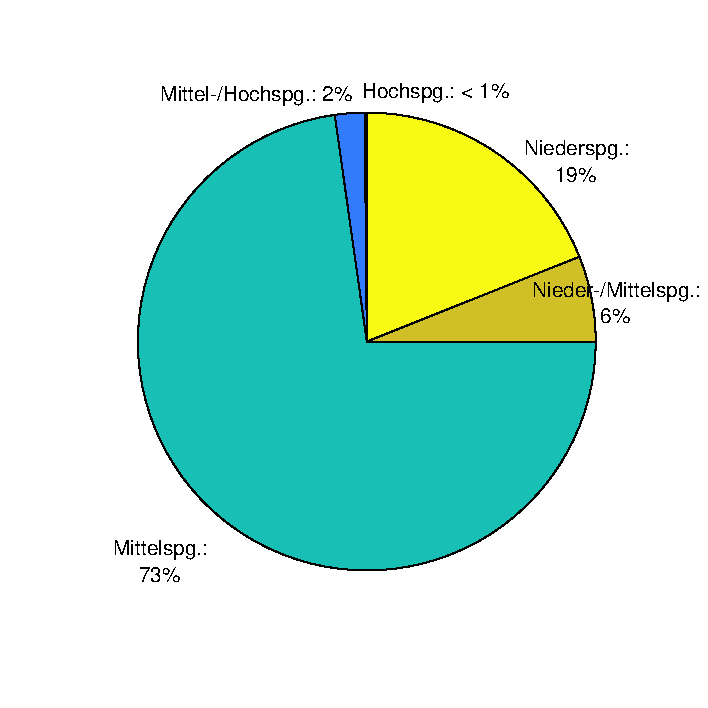
\includegraphics[width=0.4\textwidth]{img_examples/angeschNZEvert.pdf}
		%\caption[angeschlossene Netzzugangsebenen]{Über alle Datensätze betrachtet, sieht man, dass viele in der Mittel- und Niederspannung angeschlossen sind.}
		\label{fig:angeschNZEvert}} %\qquad
	\hfill
	\subfloat[Für die vorliegenden Betriebe in 2016 angewendete Leistungspreise pro Kilowatt Jahreshöchstlast.]{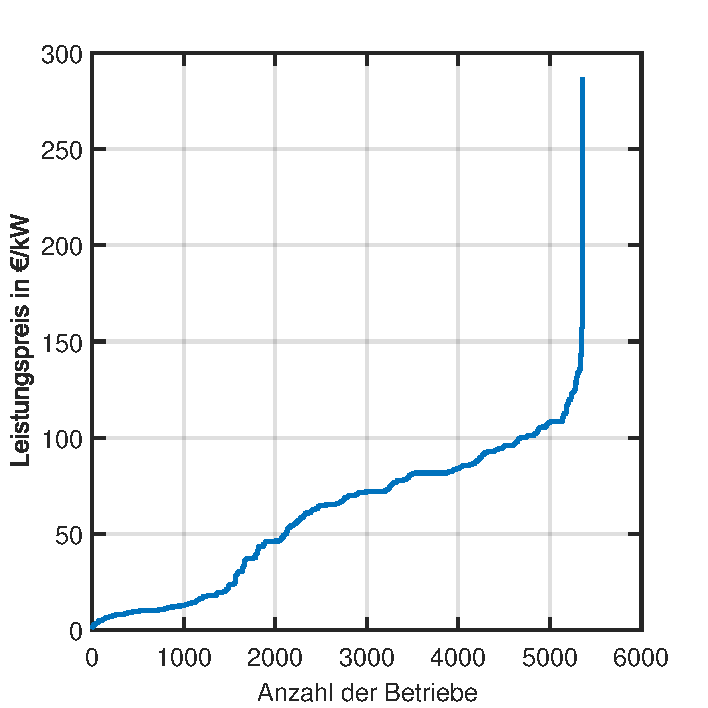
\includegraphics[width=0.4\textwidth]{img_examples/LPvert.pdf}
		%\caption[Leistungspreise über 2.500 Stunden]{Über alle Datensätze betrachtet, sieht man, dass es viele verschiedene Leistungspreise gibt.}
		\label{fig:LPvert}}
	\\
	\begin{minipage}{\textwidth}
		\subfloat[Branchenzugehörigkeit der vorliegenden Betriebe nach der Gliederung der Klassifikation der Wirtschaftszweige \cite{Branchen}.
		]{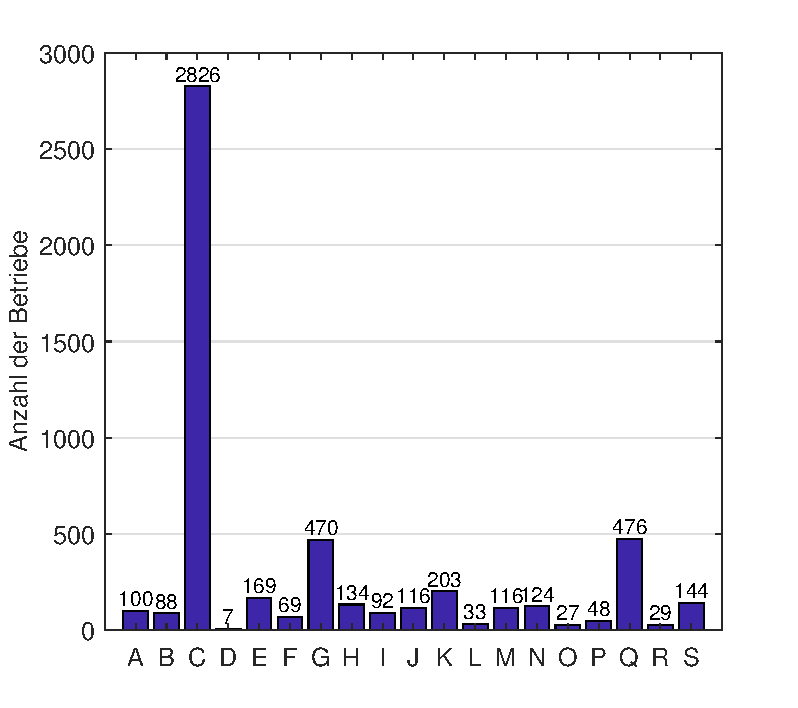
\includegraphics[width=0.5\textwidth]{img_examples/BraGrpvert.pdf}
			%\caption[Branchengruppen]{Über alle Datensätze betrachtet, sieht man, dass die meisten Firmen zum verarbeitenden Gewerbe gehören.}
			\label{fig:BraGrpvert}}
		\subfloat{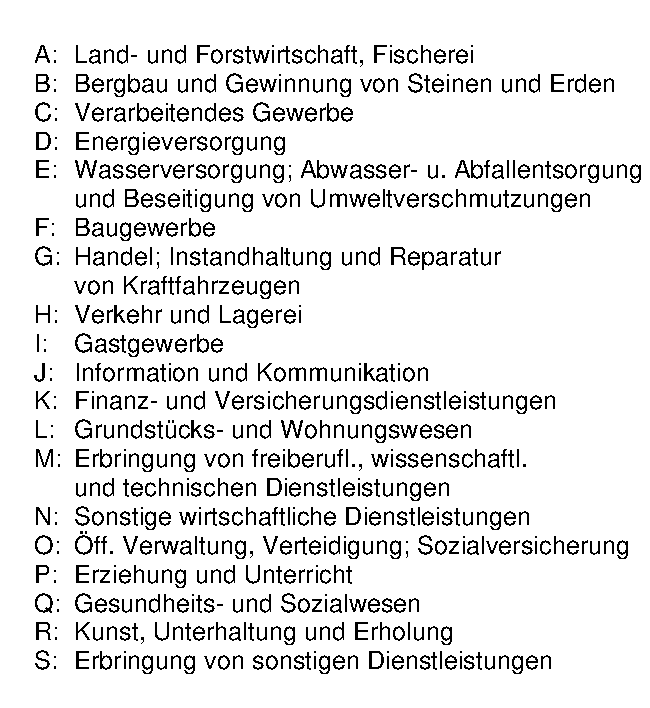
\includegraphics[width=0.45\textwidth]{img_examples/BraLabels.pdf}}
		\hfill
	\end{minipage}
	\caption[Verteilung der Betriebe auf Netzebenen, Leistungspreise und Branchen]{Beispiel für unterteilte Abbildung: Überblick über die vorliegenden Betriebe. Verteilung auf die angeschlossenen Netzebenen, die angewendeten Leistungspreise und die verschiedenen Branchen.}
	\label{fig:Verteilungen}
\end{figure}
%
Von dem Ermitteln des wirtschaftlichen Einsparpotenzials profitieren in erster Linie die Industrie und andere Unternehmen mit hohem Energiebedarf.
Sie können erfahren, unter welchen Umständen es sich für sie lohnt, in Speicher zu investieren.
Dies gilt genauso für Multiplikatoren in diesem Bereich.
Der \ac{VEA} hat gegenüber anderen Unternehmensverbänden in diesem Fall den Vorteil, dass nach Abschluss der vorgestellten Untersuchung genau bekannt ist, für welche seiner Mitglieder ein Speicher profitabel ist.
Dadurch kann er diesen gezielte Handlungsempfehlungen geben.
Die vorgestellte Untersuchung ist darüber hinaus für Akteure aus der Wissenschaft und der Speicherbranche interessant.
Unternehmen, für die ein wirtschaftlicher Speichereinsatz ermittelt wird, sind aus Sicht der Batteriehersteller potenzielle Kunden, die gezielt angesprochen werden können.
Durch Bestimmen der Kriterien, unter welchen ein Speichereinsatz für einen möglichen Kunden in Frage kommt, kann dieser leichter identifiziert und auf die Attraktivität von Speichern aufmerksam gemacht werden.
Im Rahmen einer Variation der Speicherkosten wurde beobachtet, in welchem Umfang sich die Wirtschaftlichkeit bei einer bestimmten Preisentwicklung erhöht.
Dadurch wissen Batterielieferanten, welche Kostenziele sie erreichen müssen, um neue Marktanteile zu erschlie"sen.
%
% Beispielgleichung
\begin{equation}
\label{eq:Vorl}
\Tvorl = -\tau \cdot ln \left( 1 - \frac{ 1 - \ex^{-\frac{\THLZ}{\tau}}}{\eta_{\textrm{s,cycl}}\cdot \ex^{-\frac{\THLZ}{\tau}}} \right)
\end{equation}
%
Im Folgenden wird die Systematik erklärt, wie das \ac{NNE} berechnet wird und wie es sich möglicherweise reduzieren lässt.
Außerdem wird einschlägige Literatur behandelt, die sich mit diesem und ähnlichen Themen beschäftigt.
Auf dieser Grundlage werden die Ziele dieser Arbeit definiert.
Das zweite Kapitel dient der Erklärung der verwendeten Daten, des eingesetzten Simulationsprogramms und der Wirtschaftlichkeitsberechnung.
Danach verzweigt sich die Erörterung entsprechend der genannten Ansätze.
Die zwei folgenden Kapitel behandeln eine Reduzierung der Netzentgelte mit den dafür genutzten Methoden, deren Ergebnissen und geben eine Auswertung mit anschlie"sender Diskussion.
Als erstes wird dabei die Spitzenlastkappung, der Basisfall, behandelt, und anschlie"send in Kapitel~4 die Ausnahmeregelungen nach §~19~\ac{StromNEV} erörtert.
Das letzte und fünfte Kapitel fasst die Ergebnisse zusammen und bietet einen Ausblick auf mögliche weitere Schritte.
%
\begin{table}[tb!]
	\begin{center}
			\caption{Beispiel für eine Tabelle, mit dem zugehörigen Text über der Tabelle (anders als bei Abbildungen)}
		\begin{tabular}{|c|c|}
			\hline  \thead{Information} & \thead{Wert} \\
			\hline	Betriebs-ID & 60880 \\
			\hline	Netzzugangsebene & Mittelspg. (5) \\
			\hline	Netzbetreiber &  Stadtwerke Glückstadt GmbH \\
			\hline  Arbeitspreise & \begin{tabular}{p{2cm}p{2.4cm}}\hfill <2.500~h: & \hfill 6,07~ct/kWh \\ \hfill $\geq$2.500~h: & \hfill 0,43~ct/kWh \end{tabular} \\
			\hline  Leistungspreise & \begin{tabular}{p{2cm}p{2.4cm}}\hfill <2.500~h: & \hfill 11,79~\euro/kW \\ \hfill $\geq$2.500~h: & \hfill~152,93~\euro/kW \end{tabular} \\
			\hline
		\end{tabular}
	\end{center}
	\label{tab:60880}
\end{table}
 
% ---------------------------- APPENDIX ---------------------------------------
\newpage
\appendix
\chapter{Anhang}




%--------------------------- Lists --------------------------------------------

% LISTS
\listoffigures
\listoftables

%\begin{minipage}{\textwidth}
%\lstlistoflistings
%\end{minipage}


% -------------------------- Literaturliste -----------------------------------
\newpage
\bibliographystyle{bib/bmc-des} % Style BST file (bmc-mathphys)
%\bibliographystyle{alpha}
%\bibliographystyle{abbrvdin}
\bibliography{bib/Literature.bib}

% -------------------------- Todos --------------------------------------------
\listoftodos

% -------------------------- STATEMENT ----------------------------------------
\newpage
%\thispagestyle{empty}
\begin{abstract}
	\begin{center}
		\Large{\textbf{\iflanguage{ngerman}{Erklärung}{Statement of Originality}}}\\
	\end{center}
	~\\
	\iflanguage{ngerman}{Ich versichere an Eides statt, dass ich die vorliegende \documenttype{} selbstständig verfasst und keine anderen als die angegebenen Quellen und Hilfsmittel benutzt und die allgemeinen Prinzipien wissenschaftlicher Arbeit und Veröffentlichungen, wie sie in den Leitlinien guter wissenschaftlicher Praxis der Carl von Ossietzky Universität Oldenburg festgelegt sind, befolgt habe. 
	Diese Arbeit hat in gleicher oder ähnlicher Form noch keiner Prüfungsbehörde vorgelegen.}
	{I hereby confirm in lieu of oath, that I have written the accompanying thesis by myself, without contributions from any sources other than those cited in the text and acknowledgments. I certify, that I have followed the general principles of scientific work and publications as written in the guidelines of good research of the Carl von Ossietzky University of Oldenburg.
	This work has not yet been submitted to any examination office in the same or similar form. }
	\\
	\\
	\\
	\\
	\rule{\textwidth}{0.5pt}
	\\
	\documentlocation, \iflanguage{ngerman}{den}{} \documentdate \hfill \documentauthor
\end{abstract}


\end{document}
